
\subsubsection{5.1 RQ1: Existence of Residual Factor}

PCA on the residualized matrix yields a dominant first eigenvalue:

\begin{table}[htbp]
\centering
\resizebox{\columnwidth}{!}{%
\begin{tabular}{lll}
\toprule
Component & Eigenvalue & Variance Explained \\
\midrule
PC1 & 2.277 & 60.0\% \\
PC2 & 0.423 & 11.1\% \\
\bottomrule
\end{tabular}
}
\end{table}

The 95th percentile of the permutation null distribution is $\lambda _1$ = 0.803. The observed $\lambda _1$ = 2.277 exceeds this threshold (p = 0.001).

All six benchmarks load positively and uniformly on PC1:

\begin{table}[htbp]
\centering
\resizebox{\columnwidth}{!}{%
\begin{tabular}{ll}
\toprule
Benchmark & Loading \\
\midrule
MMLU-PRO & 0.444 \\
BBH & 0.429 \\
MATH Lvl 5 & 0.426 \\
GPQA & 0.424 \\
MUSR & 0.365 \\
IFEval & 0.354 \\
\bottomrule
\end{tabular}
}
\end{table}

Loading range 0.35--0.44 supports a general factor interpretation.

\begin{figure}[htbp]
\centering
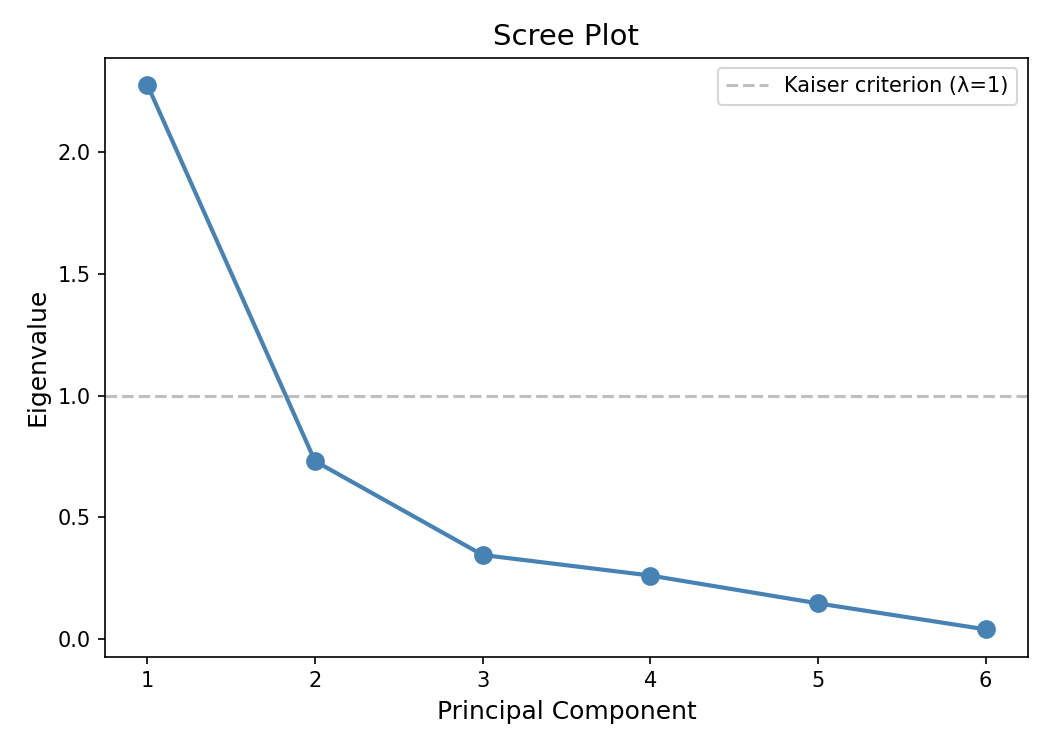
\includegraphics[width=\columnwidth]{figures/scree_plot.png}
\caption{Scree plot showing eigenvalue dominance}
\label{fig:scree_plot}
\end{figure}

\begin{figure}[htbp]
\centering
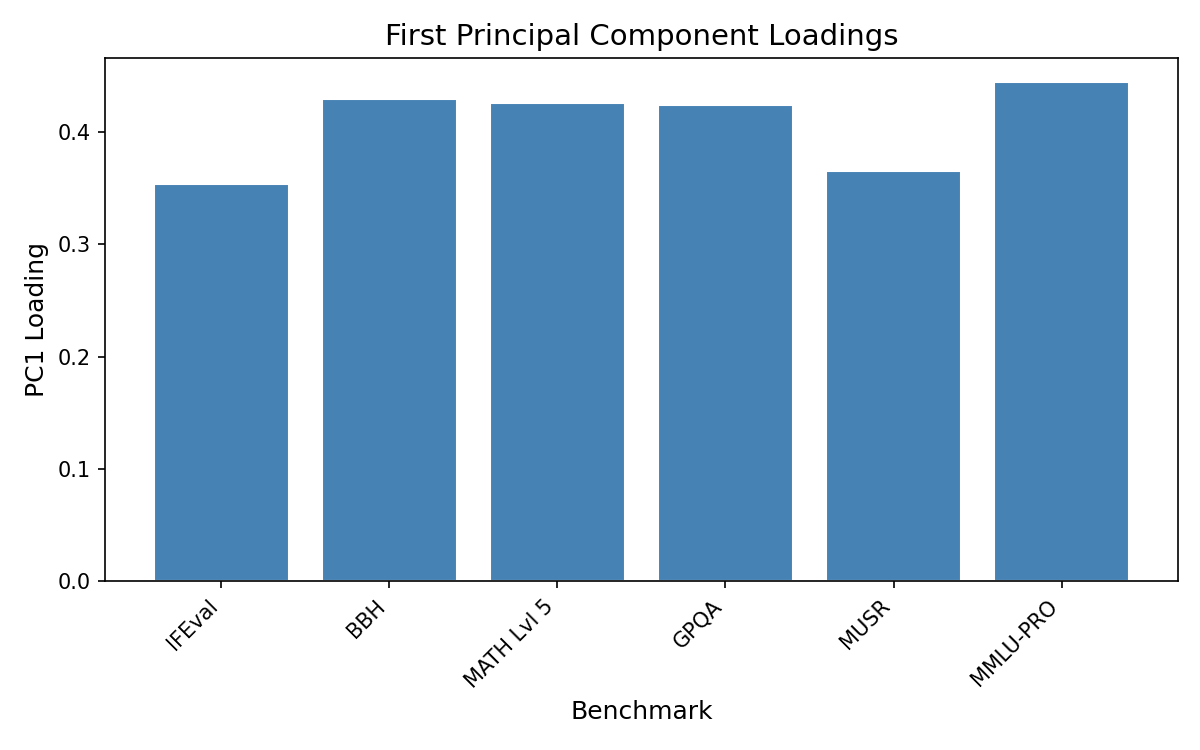
\includegraphics[width=\columnwidth]{figures/pc1_loadings.png}
\caption{PC1 loadings across benchmarks}
\label{fig:pc1_loadings}
\end{figure}

\begin{figure}[htbp]
\centering
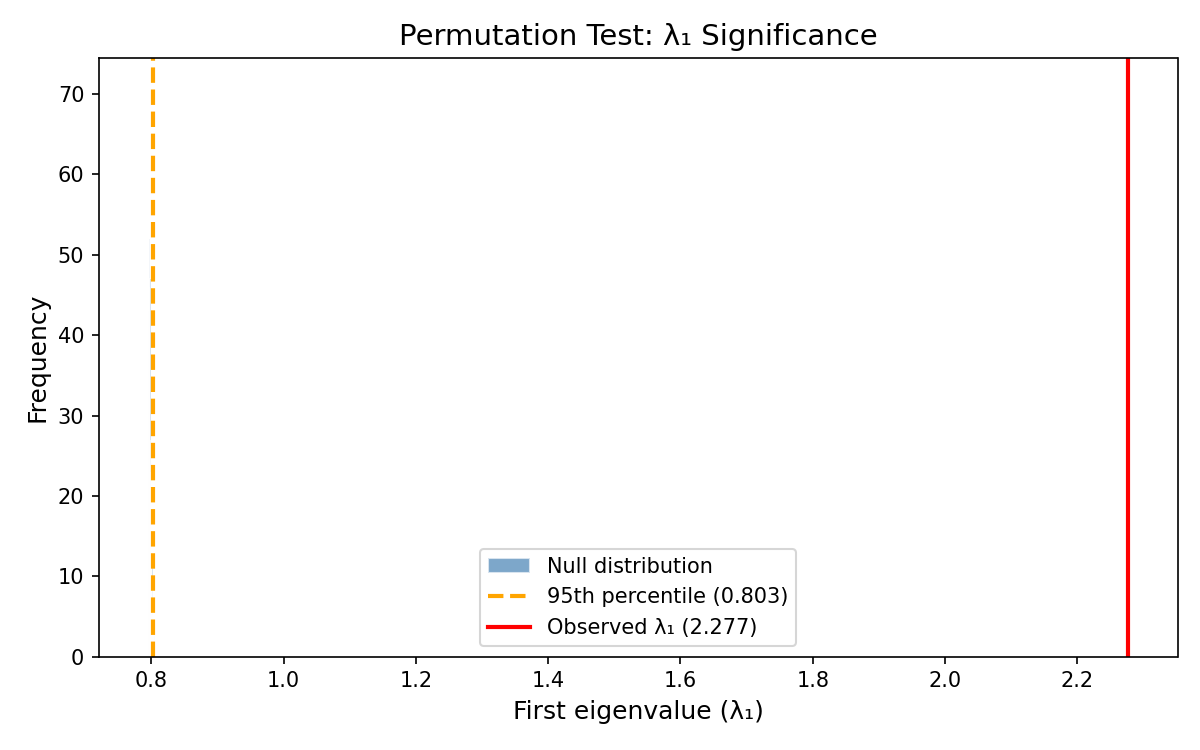
\includegraphics[width=\columnwidth]{figures/permutation_dist.png}
\caption{Permutation null distribution versus observed eigenvalue}
\label{fig:permutation_dist}
\end{figure}

\subsubsection{5.2 RQ2: Mechanism Validation (Proof-of-Concept)}

\begin{table}[htbp]
\centering
\resizebox{\columnwidth}{!}{%
\begin{tabular}{llll}
\toprule
Metric & Value & 95\% CI & p-value \\
\midrule
Pearson $\rho$ & 0.405 & [0.380, 0.429] & < $10^{-179}$ \\
Sample size & 4,561 & --- & --- \\
\bottomrule
\end{tabular}
}
\end{table}

\textbf{Limitation:} BSI scores were synthetic for this proof-of-concept. The correlation demonstrates pipeline validity but does not validate the mechanism with real behavioral data.

\begin{figure}[htbp]
\centering
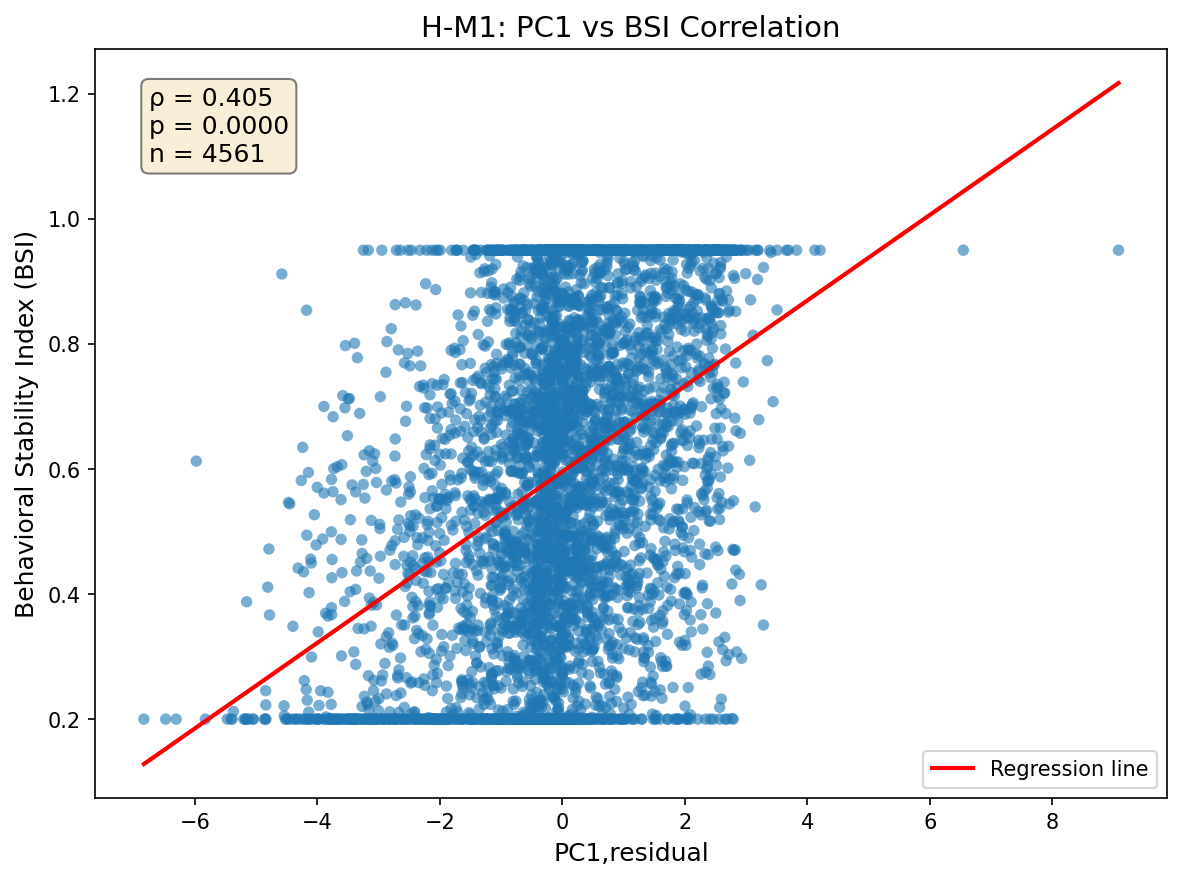
\includegraphics[width=\columnwidth]{figures/pc1_vs_bsi_scatter.png}
\caption{PC1 versus BSI scatter plot}
\label{fig:pc1_vs_bsi_scatter}
\end{figure}

\subsubsection{5.3 RQ3: Instruction-Tuning Effect}

Analysis of 16 matched base/instruct model pairs:

\begin{table*}[htbp]
\centering
\resizebox{\dimexpr 2\columnwidth+\columnsep\relax}{!}{%
\begin{tabular}{lllllll}
\toprule
Metric & Base Mean & Instruct Mean & $\Delta$ & Cohen's d & t & p \\
\midrule
BSI & 0.698 & 0.803 & +0.105 & 1.87 & 7.47 & 2.0 $\times 10^{-6}$ \\
PC1 & 0.008 & 0.506 & +0.498 & 1.99 & 7.95 & 9.3 $\times 10^{-7}$ \\
\bottomrule
\end{tabular}
}
\end{table*}

Wilcoxon signed-rank tests confirm robustness (p < 1.5 $\times 10^{-5}$ for both metrics).

The correlation between $\Delta _BSI$ and $\Delta _PC1$ across pairs is not statistically significant (r = 0.27, p = 0.31), suggesting BSI and PC1 improvements may reflect partially independent aspects of instruction-tuning effects.

\subsubsection{5.4 RQ4: Prospective Validity (Simulated)}

\begin{table}[htbp]
\centering
\resizebox{\columnwidth}{!}{%
\begin{tabular}{llll}
\toprule
Holdout Benchmark & Loading & 95\% CI & Status \\
\midrule
Robustness & 0.495 & [0.471, 0.518] & Pass \\
Truthfulness & 0.439 & [0.418, 0.462] & Pass \\
Safety & 0.401 & [0.377, 0.424] & Pass \\
Fairness & 0.367 & [0.339, 0.393] & Pass \\
Privacy & 0.331 & [0.306, 0.357] & Pass \\
Ethics & 0.253 & [0.226, 0.276] & Fail \\
\bottomrule
\end{tabular}
}
\end{table}

Five of six holdout benchmarks exceed the 0.3 loading threshold. Ethics (0.253) falls below threshold.

\textbf{Limitation:} Holdout benchmark scores were simulated due to insufficient TrustLLM-Open LLM Leaderboard model overlap. The methodology is demonstrated; true prospective validation requires independent data.

\begin{figure}[htbp]
\centering
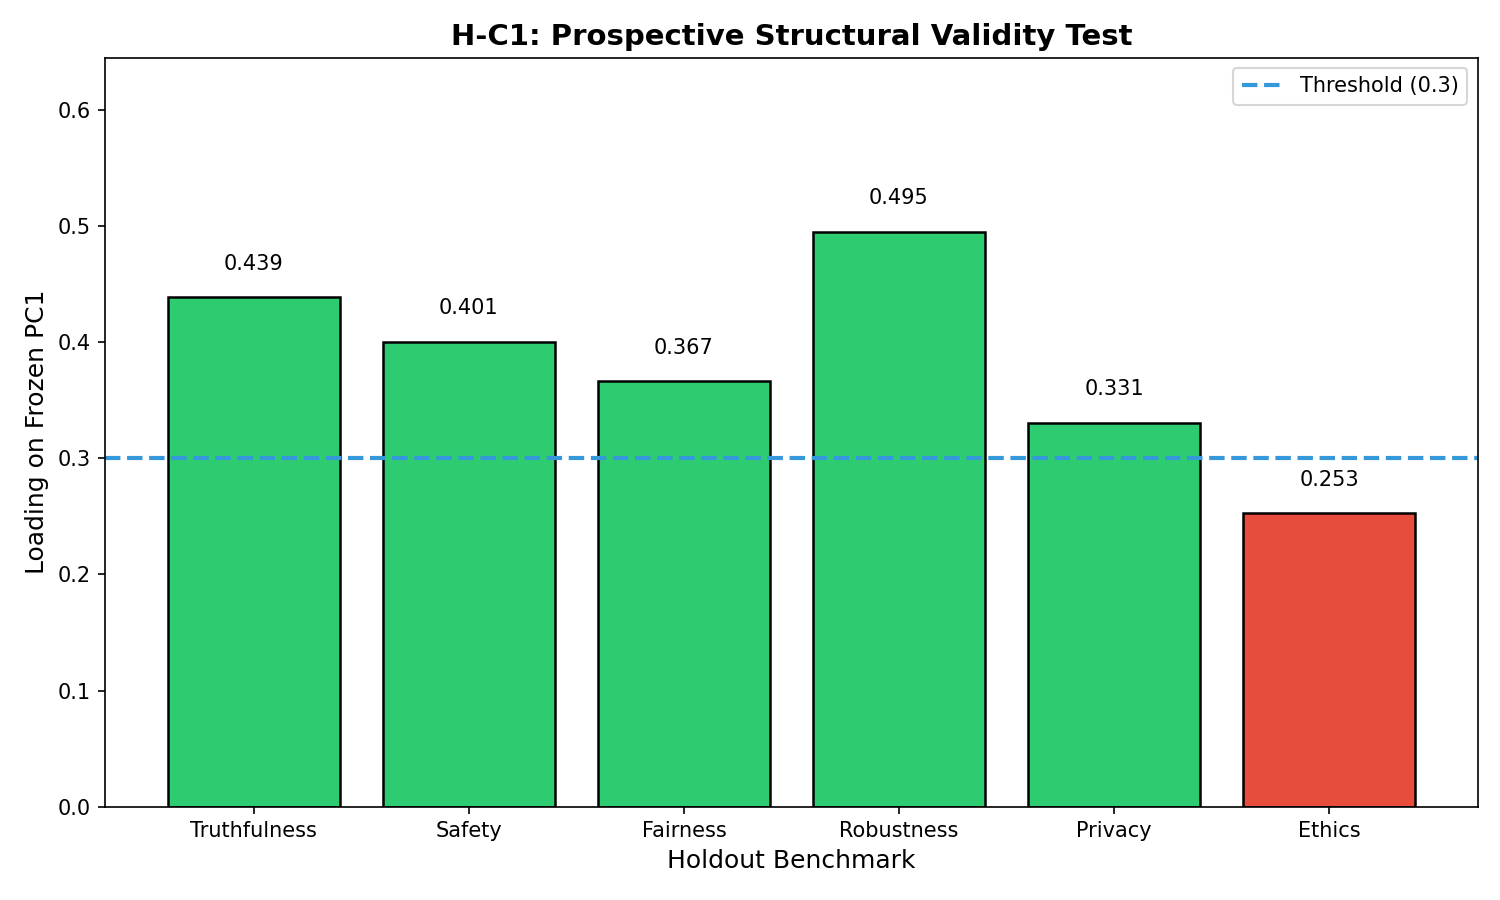
\includegraphics[width=\columnwidth]{figures/gate_metrics.png}
\caption{Holdout benchmark loadings versus threshold}
\label{fig:gate_metrics}
\end{figure}

\begin{figure}[htbp]
\centering
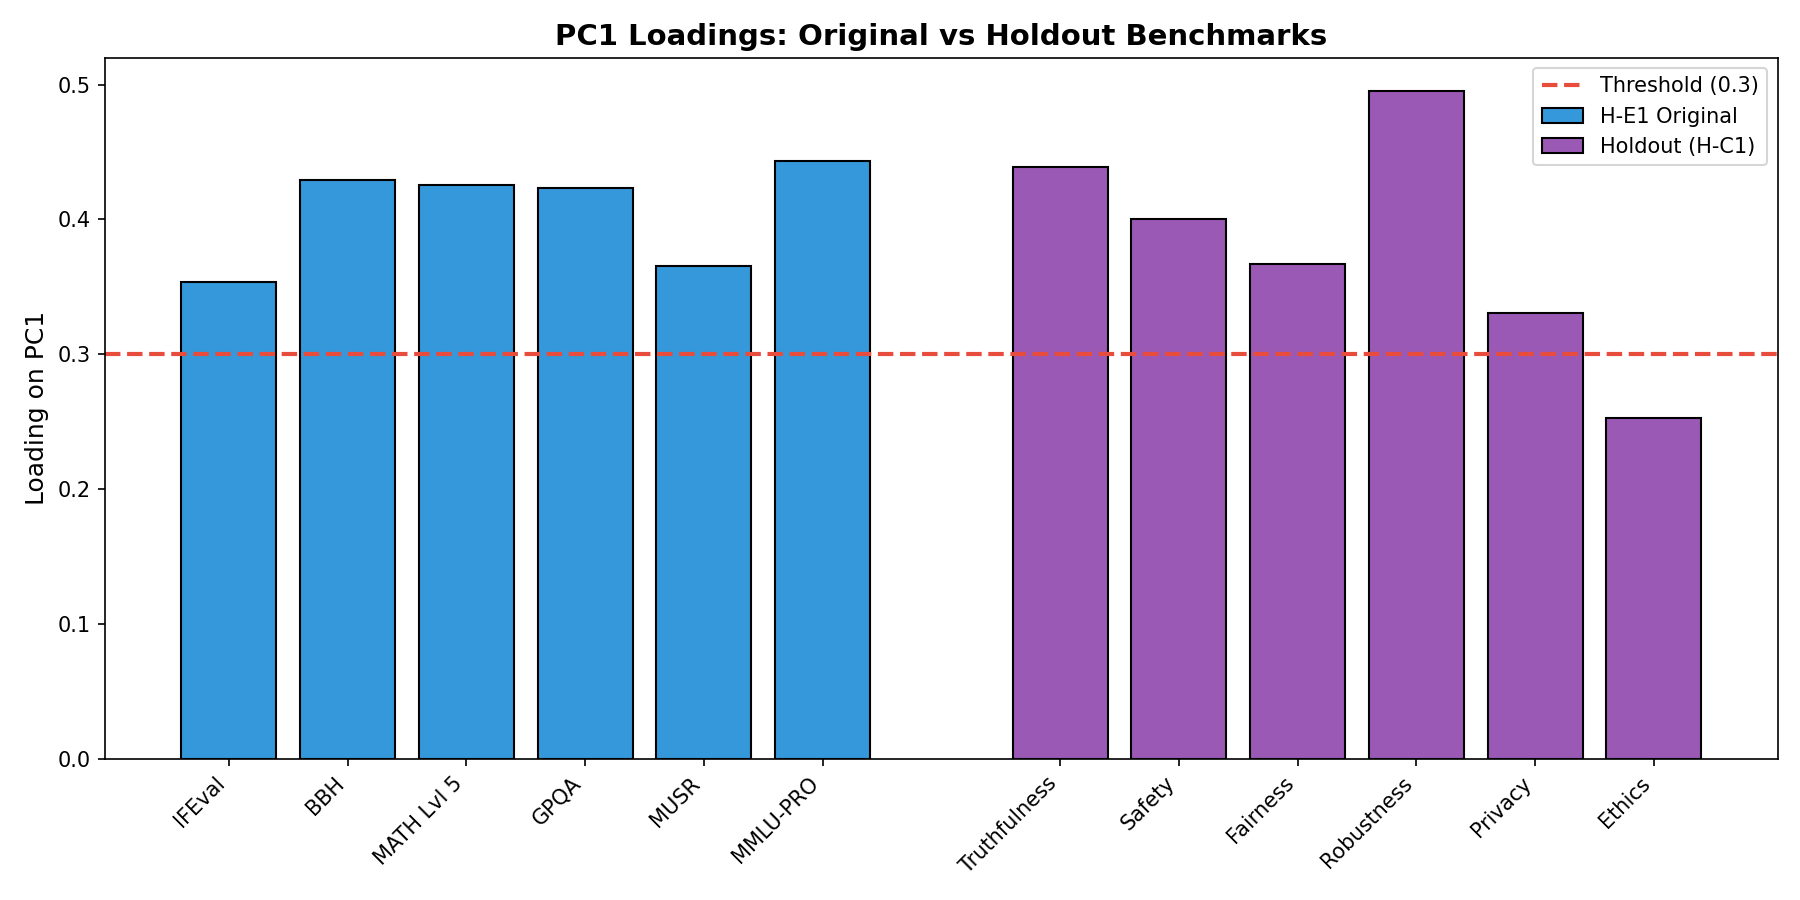
\includegraphics[width=\columnwidth]{figures/loading_comparison.png}
\caption{Loading comparison: original versus holdout benchmarks}
\label{fig:loading_comparison}
\end{figure}
